%===================================== CHAP 5 =================================

\chapter{Results}

This chapter provides all final results yielded by the the questionnaires, and the offline experiment of the CBRS as well as a discussion and analysis of the data. The chapter first lists the tables and diagrams which displays the results before discussing them.

\section{Questionnaire 1: Motivational factors}
The result from questionnaire 1 was primarily used to weight the different attributes in the CBR model, see section \ref{sec:weighting}. However it also provided to be a valuable resource as a general motivational study, therefore it will be used in the evaluation of the system. 

The questionnaire had 84 participants, with 36 answers to the open ended question on other motivational factors for choosing a location for their exchange study. All of the answers included a numerical rating between 1-7, describing how important they think each of the attribute in the questionnaire was, where these attributes represents the attributes in a case-model. Table \ref{tab:attribute_ranking} shows the values for each attribute scaled to a range between 1-10, while appendix \ref{appendix:word_frequency} displays the most frequent category of words in the textual answers.

\begin{table}[H]
\small
\caption{Statistical results from the questionnaire, 84 participants. \\ *SD: Standard Deviation, CV: Coefficient of Variation}
\centering
\label{tab:attribute_ranking}
\begin{tabulary}{\textwidth}{LRRR}
\textbf{Attribute} & \textbf{Mean (1-10)} & \textbf{SD (1-10)} & \textbf{CV (0-1)} \\ \hline
Study language & 8.2 & 1.87 & 0.23 \\ \hline
Social quality & 7.02 & 1.75 & 0.25 \\ \hline
Academic quality & 7.11 & 2.12 & 0.30 \\ \hline
Administrative support and reception & 6.5 & 2.27 & 0.35 \\ \hline
Country/Continent & 6.84 & 2.45 & 0.36 \\ \hline
Quality residential & 5.27 & 1.92 & 0.36 \\ \hline
Cost of living & 5.66 & 2.13 & 0.38 \\ \hline
Climate/weather & 6.22 & 2.53 & 0.41 \\ \hline
Availability of residentials & 5.31 & 2.22 & 0.42 \\ 
\end{tabulary}
\end{table}

The attributes are ranked by lowest coefficient of variation which yields the most important attributes given the mean rating of the attribute, and the standard deviation.

\section{Questionnaire 2}
Following are the results for all of the closed questions in questionnaire 2. Each result is followed by a brief description. The section is divided into two parts; one for for the results which contribute to RQ2 (motivational effect), and one which contribute to RQ1 (suitability of CBR in this domain).

\subsection{Motivational effect}

The following tables displays the results from the questions which concerns the motivational effect Utsida may have on students in terms of applying for an exchange program.

\begin{figure}[h]

    \centering
    
    \begin{tikzpicture}[font=\small, trim axis left, trim axis right]
        \begin{axis}[
            height=5cm,
            width=8cm,
            ybar,
            bar width=20pt,
            xlabel={Degree of agreement (1-5)},
            ylabel={Number of answers},
            ymin=0,
            ytick={2,4,6,8,10,12,14},
            xtick=data,
            axis x line=bottom,
            axis y line=left,
            enlarge x limits=0.2,
            symbolic x coords={1, 2, 3, 4, 5},
            xticklabel style={anchor=base,yshift=-\baselineskip},
            nodes near coords={\pgfmathprintnumber\pgfplotspointmeta}
        ]
        
          \addplot[fill=bootstrapBlue] coordinates {
            (1, 0)
            (2, 1)
            (3, 3)
            (4, 14)
            (5, 9)
          };
        \end{axis}
    \end{tikzpicture}
    
    \caption{I think my motivation for exchange would increase if Utsida was in use}
    \label{fig:test}
    
\end{figure}

\begin{figure}[h]

    \centering
    
    \begin{tikzpicture}[font=\small, trim axis left, trim axis right]
        \begin{axis}[
            height=5cm,
            width=8cm,
            ybar,
            bar width=20pt,
            xlabel={Degree of agreement (1-5)},
            ylabel={Number of answers},
            ymin=0,
            ytick={2,4,6,8,10,12,14},
            xtick=data,
            axis x line=bottom,
            axis y line=left,
            enlarge x limits=0.2,
            symbolic x coords={1, 2, 3, 4, 5},
            xticklabel style={anchor=base,yshift=-\baselineskip},
            nodes near coords={\pgfmathprintnumber\pgfplotspointmeta}
        ]
        
          \addplot[fill=bootstrapBlue] coordinates {
            (1, 1)
            (2, 2)
            (3, 6)
            (4, 6)
            (5, 12)
          };
        \end{axis}
    \end{tikzpicture}
    
    \caption{I think it was easy to use Utsida}
    \label{fig:test}
    
\end{figure}

\begin{figure}[h]

    \centering
    
    \begin{tikzpicture}[font=\small, trim axis left, trim axis right]
        \begin{axis}[
            height=5cm,
            width=8cm,
            ybar,
            bar width=20pt,
            xlabel={Degree of agreement (1-5)},
            ylabel={Number of answers},
            ymin=0,
            ytick={2,4,6,8,10,12,14},
            xtick=data,
            axis x line=bottom,
            axis y line=left,
            enlarge x limits=0.2,
            symbolic x coords={1, 2, 3, 4, 5},
            xticklabel style={anchor=base,yshift=-\baselineskip},
            nodes near coords={\pgfmathprintnumber\pgfplotspointmeta}
        ]
        
          \addplot[fill=bootstrapBlue] coordinates {
            (1, 0)
            (2, 0)
            (3, 1)
            (4, 3)
            (5, 9)
          };
        \end{axis}
    \end{tikzpicture}
    
    \caption{I think Utsida would have simplified my application process}
    \label{fig:test}
    
\end{figure}


\begin{figure}
    \centering
    \begin{subfigure}[b]{0.4\textwidth}
        \begin{tikzpicture}[font=\small, trim axis left, trim axis right]
        \begin{axis}[
            height=5cm,
            width=7cm,
            ybar,
            bar width=20pt,
            xlabel={Degree of agreement (1-5)},
            ylabel={Number of answers},
            ymin=0,
            ytick={2,4,6,8,10,12,14},
            xtick=data,
            axis x line=bottom,
            axis y line=left,
            enlarge x limits=0.2,
            symbolic x coords={1, 2, 3, 4, 5},
            xticklabel style={anchor=base,yshift=-\baselineskip},
            nodes near coords={\pgfmathprintnumber\pgfplotspointmeta}
        ]
        
          \addplot[fill=bootstrapBlue] coordinates {
            (1, 0)
            (2, 0)
            (3, 2)
            (4, 11)
            (5, 14)
          };
        \end{axis}
    \end{tikzpicture}
        \caption{Students who have \textbf{not} participated in an exchange program}
        \label{fig:gull}
    \end{subfigure}
    ~ \qquad %add desired spacing between images, e. g. ~, \quad, \qquad, \hfill etc. 
      %(or a blank line to force the subfigure onto a new line)
    \begin{subfigure}[b]{0.4\textwidth}
        \begin{tikzpicture}[font=\small, trim axis left, trim axis right]
        \begin{axis}[
            height=5cm,
            width=7cm,
            ybar,
            bar width=20pt,
            xlabel={Degree of agreement (1-5)},
            ylabel=\empty,
            ymin=0,
            ytick={2,4,6,8,10,12,14},
            xtick=data,
            axis x line=bottom,
            axis y line=left,
            enlarge x limits=0.2,
            symbolic x coords={1, 2, 3, 4, 5},
            xticklabel style={anchor=base,yshift=-\baselineskip},
            nodes near coords={\pgfmathprintnumber\pgfplotspointmeta}
        ]
        
          \addplot[fill=bootstrapBlue] coordinates {
            (1, 0)
            (2, 1)
            (3, 0)
            (4, 8)
            (5, 4)
          };
        \end{axis}
    \end{tikzpicture}
        \caption{Students who \textbf{have} been participated in an exchange program}
        \label{fig:tiger}
    \end{subfigure}
    \caption{I think Utsida can contribute to an increased number of students who choose to participate in an exchange program}
\end{figure}


\begin{figure}
    \centering
    \begin{subfigure}[b]{0.4\textwidth}
        \begin{tikzpicture}
        \pie{10/A, 20/B, 30/C, 40/D}
        \end{tikzpicture}        
        \caption{Students who have \textbf{not} participated in an exchange program}
        \label{fig:gull}
    \end{subfigure}
    ~ \qquad %add desired spacing between images, e. g. ~, \quad, \qquad, \hfill etc. 
      %(or a blank line to force the subfigure onto a new line)
    \begin{subfigure}[b]{0.4\textwidth}
       
        \caption{Students who \textbf{have} been participated in an exchange program}
        \label{fig:tiger}
    \end{subfigure}
    \caption{I think Utsida can contribute to an increased number of students who choose to participate in an exchange program}
\end{figure}

\begin{table}[h]
\small
\centering
\caption{Results from motivational questions from students who have not been on exchange. \\ 1: Strongly disagree, 5: Strongly agree}
\label{my-label}
\begin{tabulary}{\textwidth}{|L|R|R|}
\hline
\textbf{Question} & \textbf{Mean (1-5)} & \textbf{SD (1-5)} \\ \hline
I think my motivation for exchange would increase if Utsida was in use & 4.15 & 0.77 \\ \hline
I think it was easy to use Utsida & 3.96 & 1.16 \\ \hline
I think Utsida can contribute to an increased number of students who choose to do an exchange & 4.44 & 0.64 \\ \hline
\end{tabulary}
\end{table}

\begin{table}[h]
\small
\centering
\caption{Results from motivational questions from students who have been on 
exchange \\ 1: Strongly disagree, 5: Strongly agree}
\label{my-label}
\begin{tabulary}{\textwidth}{|L|R|R|}
\hline
\textbf{Question} & \textbf{Mean (1-5)} & \textbf{SD (1-5)} \\ \hline
I think Utsida would have simplified my application process & 4.62 & 0.65 \\ \hline
I think Utsida can contribute to an increased number of students who choose to do an exchange & 4.15 & 0.80 \\ \hline
\end{tabulary}
\end{table}

\begin{figure}
    \centering
    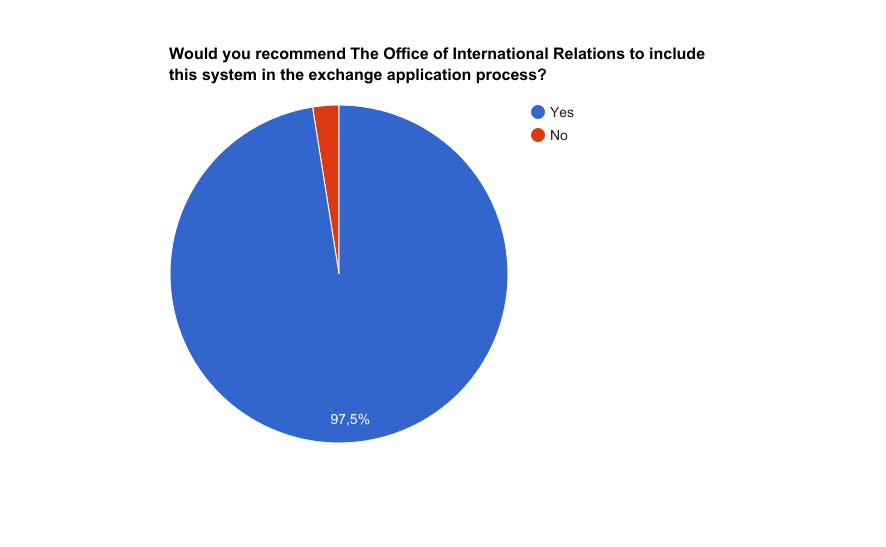
\includegraphics[width=1\textwidth]{fig/questionnaire2_diagrams/4.png}
    \caption{The ratio of \enquote{Yes} and \enquote{No}}
    \label{fig:include_system_diagram}
\end{figure}


\FloatBarrier
\subsection{Recommendation}
The following figures and tables displays the results from the questions which concerns the evaluation of the recommendations the students received with Utsida.

\subsubsection{Free search}

The first questions targeted an evaluation of the recommendations the students received with a query they composed themselves.

\begin{figure}[H]
    \centering
    \begin{subfigure}[b]{0.41\textwidth}
        \caption{Question: Did the system recommend one or more universities which are relevant for you?}
        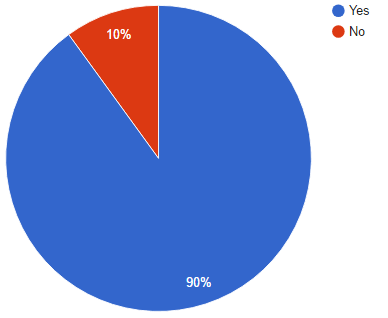
\includegraphics[width=\textwidth]{fig/results/recommendation_1.PNG}
        \label{fig:gull}
    \end{subfigure}
    ~ \qquad
    \begin{subfigure}[b]{0.40\textwidth}
        \caption{Question: Did the system recommend one or more courses which are relevant for you?}
        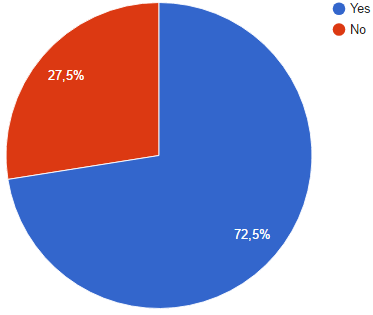
\includegraphics[width=\textwidth]{fig/results/recommendation_2.PNG}
        \label{fig:tiger}
    \end{subfigure}
    \caption{The results from the questions regarding relevancy of the students' own query}\label{fig:results_recommendation}
\end{figure}

\subsubsection{Predesigned search}

The latter questions targeted an evaluation of the recommendations the students received with two queries which were predesigned by the authors.

\begin{figure}[h]
    \centering
    \begin{subfigure}[b]{0.40\textwidth}
        \caption{Question: Did the system recommend one or more universities which are relevant for you?}
        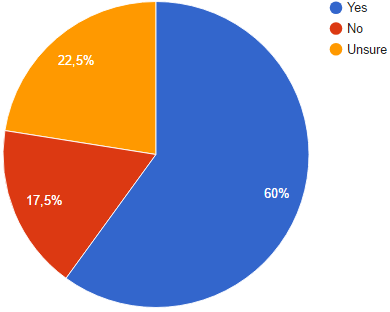
\includegraphics[width=\textwidth]{fig/results/predesigned_1.PNG}
        \label{fig:gull}
    \end{subfigure}
    ~ \qquad
    \begin{subfigure}[b]{0.40\textwidth}
        \caption{Question: Did the system recommend one or more courses which are relevant for you?}
        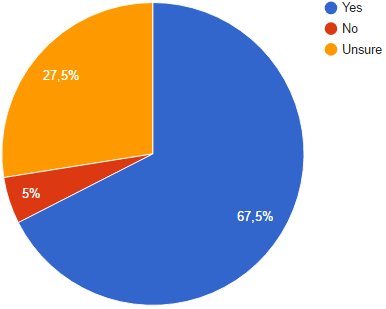
\includegraphics[width=\textwidth]{fig/results/predesigned_2.PNG}
        \label{fig:tiger}
    \end{subfigure}
    \caption{The results from the questions regarding relevancy of the students' own query}\label{fig:results_recommendation}
\end{figure}


\begin{table}[]
\centering
\caption{My caption}
\label{my-label}
\begin{tabular}{|l|l|l|}
\hline
\textbf{How suitable were the recommendations for the given query?} & \textbf{Mean (1-5)} & \textbf{SD (1-5)} \\ \hline
Query 1 & 3.93 & 0.73 \\ \hline
Query 2 & 4.03 & 0.80 \\ \hline
\end{tabular}
\end{table}






\FloatBarrier
\section{Offline Experiment of Recommender}

By using the score matrix given by table \ref{tab:offline_test}, 20 different simulated user made queries yielded the full scores seen in Appendix \ref{app:full_offline_test_results}. The central tendency results is shown in Table \ref{tab:offline_test_results}. Each query were scored on two different search models, one being Similarity based retrieval used in the CBR model and the other a simulated exact match search.

\begin{table}[H]
\centering
\caption{Results of the offline experiment, N=20}
\label{tab:offline_test_results}
\begin{tabulary}{\textwidth}{L|L|L|L|}
\cline{2-4}
                                                                           & Mean  & Std. Deviation & Std. Error Mean \\ \hline
\multicolumn{1}{|l|}{\cellcolor[HTML]{EFEFEF}Similarity based retrieval}   & 36.70 & 4.38           & .978            \\ \hline
\multicolumn{1}{|l|}{\cellcolor[HTML]{EFEFEF}Simulated exact match search} & 30.05 & 3.93           & .878            \\ \hline
\end{tabulary}
\end{table}

Table \ref{tab:offline_test_ttest} shows the Paired T-test performed on two variables from the offline experiment. The Sig. (2-tailed value) or the 2-tailed p value is lower than 0.05 indicating a that there is a significant difference between the two sample means. 

\begin{table}[H]
\centering
\caption{Results of the Paired T-test}
\label{tab:offline_test_ttest}
\begin{tabulary}{\textwidth}{ccc|c|c|ccc}
\cline{4-5}
 &  &  & \multicolumn{2}{c|}{\begin{tabular}[c]{@{}c@{}}95 \% Confidence Interval \\ of the Difference\end{tabular}} &  &  &  \\ \hline
\multicolumn{1}{|c|}{Mean} & \multicolumn{1}{c|}{\begin{tabular}[c]{@{}c@{}}Std. \\ Deviation\end{tabular}} & \begin{tabular}[c]{@{}c@{}}Std. \\ Error Mean\end{tabular} & Lower & Upper & \multicolumn{1}{c|}{t} & \multicolumn{1}{c|}{df} & \multicolumn{1}{c|}{\begin{tabular}[c]{@{}c@{}}Sig. (2-\\ tailed)\end{tabular}} \\ \hline
\multicolumn{1}{|c|}{6.65} & \multicolumn{1}{c|}{3.00} & .671 & 5.244 & 8.056 & \multicolumn{1}{c|}{9.897} & \multicolumn{1}{c|}{19} & \multicolumn{1}{c|}{0.000} \\ \hline
\end{tabulary}
\end{table}


\section{Discussion}

This section discuss the results presented in the previous sections, the limitations of the study and the recommendations based on the results. 

\subsection{Motivational effect}

Goal 1 was to "create an information system that improves the motivation for students at NTNU to go on an exchange program". This study created that information system and named it Utsida. To measure its motivational effect, and answer RQ2, a group of students were offered to test Utsida and answer a coherent questionnaire. Out of the 40 replies, 27 had not been on an exchange program before, while 13 had. For the 27 students who had not been on an exchange program, the average agreement that their motivation for exchange would increase if Utsida was in use was 4.15 out of 5, showing a strong positive influence on motivation. The standard deviation of 0.77 also shows that the answer were did not spread much from the mean, indicating that most of the participants had similar views. The average for weather they thought the system was easy to use was 3.96 out of 5, with a standard deviation of 1.16, while the average for weather they think Utsida can contribute to an increased number of students who choose to do an exchange was 4.44 out of 5, with a standard deviation of 0.64. Fir the 13 students who have all ready been on an exchange program, the average for weather they think Utsida would have simplified their application process was 4.62 out of 5, with a standard deviation of 0.65, while the average for weather they think Utsida can contribute to an increased number of students who choose to do an exchange was 4.15 out of 5, with a standard deviation of 0.80. Out of all 40 replies, 39 would recommend The Office of International Relations to include Utsida in the change application process. 

These statistics implies that the students had a positive experience of Utsida. The average response to all questions resides between \textit{4: Agree} and \textit{5: Strongly Agree}. For the students that have not been on an exchange program yet, but are interested in it, the replies suggest that Utsida would make it easier to go through the application process, and thus increasing their motivation to do so. Furthermore the replies implies that the students who have all ready been on an exchange program think they would have an easier application process. 


The results from questionnaire 1 concluded that the most important factors of motivation is the study language, social quality and academic quality, see Table \ref{tab:attribute_ranking}. These results are supported by the the results of push / pull factors of Mazzarol and Soutar \cite{mazzarol2002push}. The six most important factors identified in the study were included in the system. The open question also identified courses, information and application process as important factors, increasing the confidence in that a system like Utsida, which targets these areas, would have a positive effect on student motivation.

\subsection{Suitability of CBR methodology}

Goal 2 was to "Use the CBR methodology to give relevant recommendations on exchange program universities and courses for students at NTNU". This was accomplished by converting exchange reports to cases and using the results from questionnaire 1 on motivational factors to adjust the similarities and weights of the attributes.

The offline testing performed on the CBRS system shows that using an adjusted case-based reasoning model gives improved results compared to a standard simple search, shown in Table \ref{tab:offline_test_results}. This shows that technical part of the CBR is more suitable for recommending universities and courses compared to a simple search. The T-test two-tailed p value of less than 0.05 also shows that there is a significant difference in means between the two samples.  

A high number of the participators in questionnaire 2 answered that they were given relevant recommendations to universities and courses. This answers RQ1 and shows that it is feasible to use CBR to recommend courses and universities.

\subsection{Limitations}
Some limitations of this project was present. The most important factor being the sample size of the population for questionnaires. While both questionnaires got a decent amount of answer;  questionnaire 1 with 84 answers and questionnaire 2 with 40 answers. This number of participant should be even larger to be able to conclude with a definite result. The result data did however trend highly positive with average responses to all questions residing between \textit{4: Agree} and \textit{5: Strongly Agree}. Furthermore, to avoid even more bias, the questionnaires should have undergone more rigorous pilot testing with experts on the field of questionnaire design, this was not possible due to time limits and cost. 

\subsection{Recommendations}
Based on the results that show a high positive attitude towards the system this study highly recommends that NTNU invest further in digitalising the whole or part of the application process for exchange programs. The study also shows that the exchange reports submitted by students can be used for different purposes than just searching through. Therefore it is recommended that the data from the experience reports should be open to use so that students and others can utilize them in ways that may give a benefit to NTNU. 



\cleardoublepage